\documentclass[10pt,a4paper]{article}
\usepackage[utf8]{inputenc}
\usepackage[T1]{fontenc}
\usepackage{lmodern}
\usepackage[margin=1.5cm, top=1.4cm, bottom=1.4cm]{geometry}
\usepackage{hyperref}
\usepackage{enumitem}
\usepackage{titlesec}
\usepackage{xcolor}
\usepackage{graphicx}

\definecolor{accent}{HTML}{00686E}
\hypersetup{colorlinks=true, urlcolor=accent, linkcolor=accent}
\pagenumbering{arabic}
\setlength{\parindent}{0pt}

\titleformat{\section}{\large\bfseries\color{accent}}{}{0em}{}[\vspace{-0.6em}\rule{\textwidth}{0.8pt}]
\titlespacing{\section}{0pt}{7pt}{4pt}

\newcommand{\role}[4]{%
  \textbf{#1} \hfill \textbf{#2}\\[1pt]%
  \textit{#3} \hfill \textit{#4}\\[2pt]%
}
\setlist[itemize]{leftmargin=1.2em, itemsep=1.5pt, topsep=2pt, parsep=0pt}

\begin{document}

% ================= HEADER =================
\begin{minipage}[c]{0.80\textwidth}
  {\Huge\bfseries Prabhavit Gupta}\\[3pt]
  {\color{accent}\large Principal AI \& Analytics Engineer: Reporting Platforms \& AI-Driven Engineering}\\[6pt]
  {\footnotesize +39 351 610 7807 ~$\vert$~
  \href{mailto:prabhavitg@gmail.com}{prabhavitg@gmail.com} ~$\vert$~
  \href{https://www.linkedin.com/in/prabhavit/}{linkedin.com/in/prabhavit} ~$\vert$~
  \href{https://github.com/prab-gupta}{github.com/prab-gupta} ~$\vert$~
  Venice, Italy (CET Time Zone / EU Permanent Resident / Available Immediately)}
\end{minipage}\hfill
\begin{minipage}[c]{0.18\textwidth}
  \raggedleft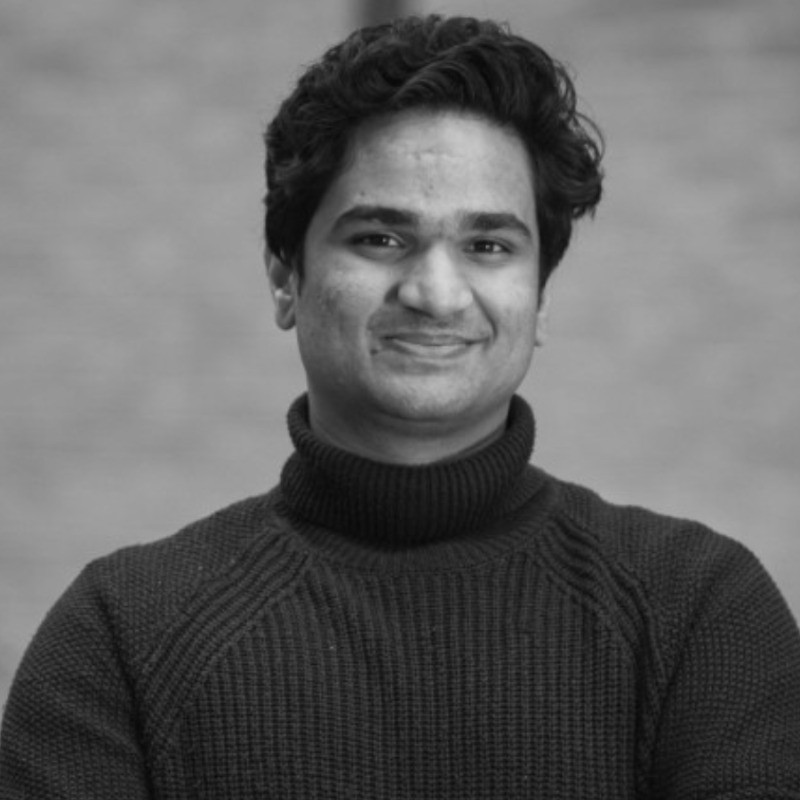
\includegraphics[width=2.0cm]{photo.jpg}
\end{minipage}
\vspace{-2pt}

% ================= SUMMARY =================
\section{Summary}
Hands-on Principal AI and Analytics Platform Engineer with 3 years of commercial software engineering experience architecting high-performance reporting systems, analytical data models, and modern multi-tenant SaaS data platforms. Pioneer in leveraging AI coding tools (Claude Code, Cursor) to automate and accelerate end-to-end software delivery from greenfield design to production release. Proven track record designing self-service report builders, optimizing high-volume PostgreSQL analytical queries, enforcing strict tenant isolation, and implementing automated data reconciliation test suites. Based in Venice, Italy (CET time zone) with an EU Long-Term Residence Permit (permanent unrestricted EU work authorization across all EU member states, no sponsorship required); available immediately for full-time remote roles.

% ================= TECHNICAL EXPERTISE =================
\section{Technical Expertise}
\begin{itemize}
  \item \textbf{Analytics \& Reporting Architecture:} Self-service reporting engines, dimensional data modeling, aggregation pipelines, metrics catalogs, SQL query optimization, automated data reconciliation test suites.
  \item \textbf{AI-Accelerated Software Development:} Claude Code autonomous workflows, Cursor AI pair programming, Model Context Protocol (MCP) tool integration, prompt regression testing.
  \item \textbf{Backend \& Cloud Systems:} Python (FastAPI, asyncio, Pydantic), TypeScript/Node.js, PostgreSQL (partitioning, indexing, tenant schema isolation), AWS cloud services, Redis in-memory caching.
  \item \textbf{Multi-Tenant Security \& Reliability:} Strict tenant isolation, role-based access control (RBAC), audit logging, zero-downtime database migrations, 99.8\% production SLA maintenance.
  \item \textbf{Testing \& Observability:} End-to-end regression testing with pytest and Playwright, Prometheus telemetry, structured logging, CI/CD with GitHub Actions.
  \item \textbf{Languages \& Authorization:} English (C1 Professional, fluent), Hindi (Native), Italian (Conversational). EU Long-Term Residence Permit (unrestricted EU work authorization, no sponsorship required). Available immediately.
\end{itemize}

% ================= EXPERIENCE =================
\section{Experience}

\role{\href{https://flowspace.co}{FlowSpace.co}}{Mar 2024 - Aug 2026}{Lead Analytics \& AI Systems Engineer}{London, UK (remote)}
\begin{itemize}
  \item Designed and delivered the core analytical data pipeline and customer reporting infrastructure serving 4,500+ enterprise users with sub-second report generation.
  \item Accelerated full-stack platform development using Claude Code and Cursor, authoring automated test suites, schema migrations, and REST APIs at 3x standard velocity.
  \item Architected multi-tenant PostgreSQL data models with strict tenant isolation, decreasing analytical query p95 latency by 42\% through strategic composite indexing.
  \item Built automated data reconciliation engines comparing transactional source tables against materialized reporting aggregates to guarantee 100\% metric fidelity.
  \item Deployed containerized microservices and automated CI/CD workflows on cloud infrastructure, sustaining 99.8\% availability across continuous release cycles.
\end{itemize}

\role{Urlink}{Apr 2025 - Jul 2025}{Analytics Platform Developer (Freelance)}{Barcelona, Spain (remote)}
\begin{itemize}
  \item Implemented automated data ingestion and reporting transformations extracting structured operational metrics into centralized analytical stores.
  \item Built automated regression and data integrity test suites with pytest and Playwright to validate calculated KPIs against benchmark operational datasets.
  \item Developed custom export utilities allowing enterprise stakeholders to schedule and download self-service CSV and PDF reports.
\end{itemize}

\role{Independent Technical Consultant}{Aug 2023 - Feb 2024}{Data Systems \& Software Engineer}{Venice, Italy}
\begin{itemize}
  \item Designed and deployed custom reporting dashboards and ETL microservices for European SMB clients, automating manual spreadsheet reporting workflows.
  \item Built optimized SQL queries and database migration pipelines in Python for multi-tenant customer management applications.
  \item Authored technical architecture runbooks and data dictionary documentation for client engineering leadership.
\end{itemize}

% ================= EDUCATION =================
\section{Education}
\role{Ca' Foscari University of Venice}{2020 - 2024}{BA in Philosophy, International Studies and Economics}{Venice, Italy}
\begin{itemize}
  \item Rigorous training in formal logic, statistical inference, quantitative economics, and complex systems modeling.
\end{itemize}

\end{document}
